\documentclass{article}

% NeurIPS 2026 template
\usepackage[preprint]{neurips_2026}

\usepackage[utf8]{inputenc}
\usepackage[T1]{fontenc}
\usepackage{hyperref}
\usepackage{url}
\usepackage{booktabs}
\usepackage{multirow}
\usepackage{graphicx}
\usepackage{microtype}
\usepackage{xcolor}
\usepackage{amsmath,amssymb}

\title{Useful but Not Revealing: Privacy-Aware Visual Token Pruning
for Vision-Language Models}

\author{
  Ahmed Abdelnaby (011922747) \\
  \texttt{ahmed.abdelnaby@wsu.edu}
  \And
  Mohamed Shaaban (011926089) \\
  \texttt{mohamed.shaaban@wsu.edu}
}

\begin{document}

\maketitle

% =========================================================
\begin{abstract}
Vision-language models (VLMs) represent an image as a set of visual tokens that are processed together with a user's question.
Only some of these tokens are needed to answer a given question, yet the rest can still encode private information such as
faces, names, identity documents, addresses, or license plates. Existing visual-token pruning methods remove tokens to save
computation and do not consider whether the retained tokens expose private content. We propose a privacy-aware pruning
framework that scores every visual token by its \emph{task relevance} to the current question and its \emph{privacy risk},
and keeps the top-$K$ tokens of $S_i = R_i - \lambda P_i$. A 0.27M-parameter privacy predictor is trained on frozen visual
features using pixel-level VISPR redaction annotations; the VLM (LLaVA-1.5-7B) stays frozen. On 200 VISPR test images and
300 GQA questions, we find that (i) relevance-only pruning, the basis of existing pruners, \emph{preferentially} retains
private tokens; (ii) privacy-aware selection at half the token budget reduces adversarial attribute leakage from 0.72 to 0.54
with no loss of GQA accuracy, and to 0.30 at a 4-point cost; (iii) the learned predictor protects better than the ground-truth
masks themselves, because private information spreads into neighbouring tokens; and (iv) removing tokens does not remove
information: private attributes remain linearly recoverable from the kept tokens. Privacy-aware pruning is therefore an
effective, zero-cost first line of defence, but not a privacy guarantee.
\end{abstract}

% =========================================================
\section{Introduction}

Vision-language models have demonstrated strong performance on multimodal tasks such as image understanding, visual question
answering, and instruction following. Models such as LLaVA combine a pretrained vision encoder with a large language model,
representing an image as visual tokens that are processed together with natural-language instructions~\cite{liu2024improved}.
This architecture raises a privacy concern: the language model receives visual information that may be unnecessary for
answering the user's question.

Consider an image of a person standing beside a car whose license plate is visible, and the question ``What color is the
car?'' The regions containing the person's face and the license plate are not needed to answer it, yet a conventional VLM
processes them anyway. Personal images contain many such attributes, including faces, names, addresses, documents, and
signatures~\cite{orekondy2017towards}, and VLMs can infer them at scale~\cite{tomekce2024private}. When inference is split
between a device and a cloud server, every visual token sent to the server is a potential leak.

At the same time, many of the visual tokens a VLM processes are redundant. Visual-token pruning methods remove less useful tokens
to reduce computational cost~\cite{chen2024imageworth12tokens,pmlr-v267-zhang25s,Zhang_2025_ICCV,alvar2025divprune}.
They optimise efficiency and task accuracy, and do not consider whether the retained tokens are private.

We investigate whether visual-token pruning can serve a second purpose: protecting privacy. We score each visual token by two
complementary properties. \emph{Task relevance} measures how useful the token is for the current question; \emph{privacy risk}
estimates whether it contains sensitive information. Selecting tokens that are relevant and low-risk aims to keep what the
task needs while withholding private content, at no additional inference cost, since the pruned model is also faster.

\textbf{Contributions.}
\begin{itemize}
\item A prompt-conditioned, privacy-aware token selection method for frozen VLMs, with a lightweight token-level privacy predictor
trained from pixel-level redaction masks (Sec.~\ref{sec:method}).
\item An evaluation protocol that measures privacy in three complementary ways: geometric (private tokens retained), behavioural
(whether the model can still confirm a private attribute, including under adversarial questions), and representational (whether the
attribute is recoverable from the kept tokens) (Sec.~\ref{sec:setup}).
\item Empirical findings (Sec.~\ref{sec:results}): attention-based pruning retains private content preferentially; privacy-aware selection
removes much of the leakage at little or no utility cost; leakage is partly located in tokens \emph{around} the annotated regions, so a
graded, learned risk score beats the ground-truth masks; and token removal alone leaves private attributes recoverable.
\end{itemize}

% =========================================================
\section{Related work}

\textbf{Vision-language models.} LLaVA connects a pretrained CLIP vision encoder to a large language model through a small projector
and is trained for visual instruction following~\cite{liu2024improved}. CLIP learns aligned visual and textual representations from
large-scale image--text data~\cite{radford2021learning}. In these architectures an image becomes a grid of visual tokens before language
generation, which is the representation we operate on.

\textbf{Visual token pruning.} FastV observes that many visual tokens receive little attention during VLM inference and removes them
after an early layer~\cite{chen2024imageworth12tokens}. SparseVLM performs text-guided visual token sparsification~\cite{pmlr-v267-zhang25s}.
VisPruner questions whether text--visual attention alone is reliable for token selection and uses visual cues instead~\cite{Zhang_2025_ICCV}.
DivPrune keeps a diverse subset of tokens~\cite{alvar2025divprune}. These methods show that VLM visual representations are highly redundant,
but they optimise computational cost and accuracy only. Our relevance term is interchangeable with their scores; our contribution is the privacy
term and the measurement of what pruning does to privacy. Our results add a cautionary observation about attention-based pruners: because
VLM attention concentrates on people and text, these pruners keep private content preferentially.

\textbf{Visual privacy.} VISPR introduced a taxonomy and dataset of privacy-sensitive image attributes~\cite{orekondy2017towards}. Follow-up work
added pixel-level annotations for localisable attributes and showed that redacting these regions gives privacy while retaining utility
\emph{for human viewers}~\cite{orekondy2018connecting}. Pixel-level obfuscation such as blurring or pixelation can be defeated by learned
models~\cite{mcpherson2016defeating}, which motivates studying privacy at the representation level. We redact \emph{tokens} for a \emph{model},
conditioned on the question, and find that masks sufficient for human viewers leave attributes recoverable by the model.

% =========================================================
\section{Method}\label{sec:method}

Figure~\ref{fig:method} illustrates the framework: visual token extraction, task relevance estimation, privacy risk estimation, and
privacy-aware token selection. Only the privacy predictor is trained; the VLM remains frozen.

\begin{figure}[t]
    \centering
    \includegraphics[width=\linewidth]{figs/methodology.png}
    \caption{Overview of privacy-aware visual token pruning. A frozen vision encoder turns the image into visual tokens. Task relevance
    identifies tokens useful for the current question, and a lightweight privacy predictor estimates which tokens contain sensitive
    information. The two signals select a smaller set of task-relevant, low-risk tokens before language generation. The privacy predictor
    is trained offline on localised privacy annotations from VISPR.}
    \label{fig:method}
\end{figure}

\subsection{Visual token extraction}
We use LLaVA-1.5-7B~\cite{liu2024improved}. The image is padded to a square and resized to $336^2$, and CLIP ViT-L/14-336 produces
$N{=}576$ patch features $z_i\in\mathbb{R}^{1024}$ (second-to-last layer, a $24{\times}24$ grid), which a two-layer projector maps to
language-model embeddings $v_i$. To prune, we build the language-model input ourselves as \texttt{[prompt prefix | $v_i$ for $i\in\mathcal{K}$ | question]},
keeping the selected tokens in their original raster order; dropped tokens are never seen by the language model. With $\mathcal{K}$ equal to all
tokens, this reproduces the reference implementation exactly (maximum logit difference 0.0). We disable the default centre crop of the public
LLaVA processor, which would cut off part of non-square images and misalign tokens with the privacy annotations.

\subsection{Task relevance estimation}
Relevance is conditioned on the question. Our main estimator uses the VLM's own attention: we run the first 16 language-model layers on the full
sequence and average the attention from the question tokens $Q$ to visual token $i$ over layers $\mathcal{L}=\{2,\dots,15\}$ and all heads $H$,
\begin{equation}
\tilde R_i = \frac{1}{|\mathcal{L}|\,|H|\,|Q|}\sum_{l\in\mathcal{L}}\sum_{h\in H}\sum_{t\in Q} A^{l,h}_{t,i}.
\end{equation}
As an alternative that needs no language-model pass, we use the cosine similarity between CLIP's text embedding of the question and dense
CLIP patch features~\cite{zhou2022maskclip}. This variant matters when the language model runs on an untrusted server: computing attention-based
relevance already exposes every token to it, whereas CLIP relevance can be computed on the device. A small number of visual tokens receive far more
attention than the rest~\cite{darcet2024registers}, so min--max scaling would squash most scores toward zero and change the effective strength of
$\lambda$ from image to image. We therefore rank-normalise, $R_i=\mathrm{rank}(\tilde R_i)/(N-1)\in[0,1]$.

\subsection{Privacy risk estimation}
Privacy risk is independent of the question. We use the VISPR redaction dataset~\cite{orekondy2018connecting}, which provides polygons for 28
privacy attributes (face, person, nudity, name, address, date/time, license plate, passport, credit card, signature, handwriting, and others).
We apply the same pad-and-resize to the polygons, rasterise them at $4\times$ resolution, and pool them onto the token grid:
\begin{equation}
o_{i,c} = \frac{|A_i\cap M_c|}{|A_i|}, \qquad P^{GT}_i = \frac{|A_i\cap \bigcup_c M_c|}{|A_i|},
\end{equation}
where $A_i$ is the $14{\times}14$ patch of token $i$ and $M_c$ the mask of attribute $c$. $P^{GT}$ is the ground-truth (oracle) privacy risk
(Fig.~\ref{fig:masks}); 28.7\% of test tokens have $P^{GT}_i>0.25$.

The privacy predictor $f_P$ is LayerNorm $\to$ Linear(1024, 256) $\to$ GELU $\to$ Linear(256, 28) applied to each frozen $z_i$, with sigmoid
outputs $p_{i,c}$ (attributes overlap, e.g.\ a face lies inside a person). It is trained on the soft targets $o_{i,c}$ with class-weighted binary
cross-entropy, $w^+_c=\min(\mathrm{neg}_c/\mathrm{pos}_c,100)$, so that rare attributes such as passports are not swamped by faces and people.
The token's risk is $P_i=\max_c p_{i,c}$.

\begin{figure}[t]
\centering
\includegraphics[width=\linewidth]{figs/mask_check.png}
\caption{Token-level privacy ground truth $P^{GT}_i$ (red tint) on random VISPR test images after LLaVA's pad-and-resize; titles list the annotated attributes.
Annotated regions are pixelated for display only, one flat colour per token, so the pixelated blocks show exactly the token-level mask.}
\label{fig:masks}
\end{figure}

\subsection{Privacy-aware token selection}
With $x_i\in\{0,1\}$ indicating a kept token and a budget of $K$ tokens, we solve
\begin{equation}
\max_{x}\ \sum_i x_i R_i - \lambda \sum_i x_i P_i \quad \text{s.t.} \quad \sum_i x_i = K,
\end{equation}
whose exact solution is to keep the $K$ tokens with the highest $S_i=R_i-\lambda P_i$ (\emph{soft} selection). $\lambda=0$ recovers relevance-only
pruning, and increasing $\lambda$ traces the privacy--utility trade-off. A \emph{hard} gate instead never keeps a token with $P_i\ge\tau$, so it may keep
fewer than $K$ tokens. The distinction matters because relevance depends on the question: an adversarial question such as ``Is someone's face visible?''
pulls relevance onto exactly the private tokens, and a soft penalty can then be outweighed, whereas a hard gate cannot.

% =========================================================
\section{Experimental setup}\label{sec:setup}

\textbf{Data.} VISPR redactions~\cite{orekondy2017towards,orekondy2018connecting}: 3,873 / 1,611 / 2,989 train / validation / test images.
The privacy predictor is trained on the training split and selected on validation token AP. Evaluation uses 200 random test images.
For utility on a standard benchmark we use 300 questions from GQA testdev-balanced~\cite{hudson2019gqa}; GQA images have no privacy annotations,
so only the learned privacy predictor applies to them.

\textbf{Tasks.} For each VISPR test image we ask: (1) three privacy-neutral utility questions (scene type, indoor/outdoor, background colour);
(2) an \emph{adversarial} probe for each present attribute, the official VISPR yes/no question (e.g.\ ``Is someone's face visible?''), with relevance
computed from the probe itself, i.e.\ the attacker chooses the question; (3) a \emph{benign} probe, the same question asked after tokens were selected
for a neutral question; and (4) two probes for attributes that are \emph{absent}, to detect a model that simply answers ``yes''.
In total: 600 utility questions, 531 adversarial and 531 benign probes, and 400 absent-attribute probes.

\textbf{Baselines and grid.} All 576 tokens (full); random pruning; relevance-only pruning ($\lambda=0$); privacy-only pruning (lowest $P_i$);
soft selection with $\lambda\in\{0.1,0.25,0.5,1,2\}$; hard selection with $\tau\in\{0.5,0.8\}$. Each method is run with the oracle $P^{GT}$ and the learned $P$,
with attention and CLIP relevance, at budgets $K\in\{432, 288, 144, 58\}$ (75\%, 50\%, 25\%, 10\%). Answers use greedy decoding (at most 10 tokens).

\textbf{Metrics.}
\emph{Geometric privacy}: private-token retention $\mathrm{PTR}=\sum_i x_iP^{GT}_i/\sum_iP^{GT}_i$.
\emph{Behavioural privacy}: leakage, the ``yes'' rate on present-attribute probes (adversarial and benign); the false-``yes'' rate on absent attributes is
at most 0.10 for every configuration, so leakage is not a ``yes'' bias.
\emph{Representational privacy}: recoverability, the mAP of a linear probe trained to predict the 28 attributes from the mean of the kept tokens (chance level 0.09).
\emph{Utility}: exact agreement with the full-token answer on VISPR utility questions, and accuracy on GQA.
\emph{Efficiency}: number of visual tokens passed to the language model.
Differences are tested with paired bootstrap confidence intervals (2,000 resamples over tasks).

\textbf{Implementation.} PyTorch and Hugging Face Transformers, fp16, one NVIDIA RTX 4090. The privacy predictor trains in minutes on cached features.
The full evaluation grid takes about 40\,s per image, dominated by generating one answer for each of about 125 configurations per question.

% =========================================================
\section{Results}\label{sec:results}

\subsection{Privacy predictor}
The predictor separates private from non-private tokens with token-level AP 0.87 on the test set (validation 0.86); the mean AP over the 28 attributes is 0.48.
Quality varies strongly by attribute (Table~\ref{tab:head}): large visual categories are detected well, while text-based attributes are weak, which is expected
because 14-pixel CLIP patches do not resolve characters.

\begin{table}[h]
\centering\small
\caption{Token-level AP of the learned privacy predictor for selected attributes (test set).}
\label{tab:head}
\begin{tabular}{@{}lc lc lc lc@{}}
\toprule
Attribute & AP & Attribute & AP & Attribute & AP & Attribute & AP \\
\midrule
person & 0.91 & ticket & 0.78 & nudity & 0.61 & name & 0.39 \\
face & 0.88 & handwriting & 0.76 & license plate & 0.49 & address & 0.29 \\
passport & 0.84 & credit card & 0.73 & date/time & 0.47 & e-mail & 0.13 \\
\bottomrule
\end{tabular}
\end{table}

\subsection{Main results}
Table~\ref{tab:main} reports the main comparison, Figure~\ref{fig:budget} shows all budgets, and Table~\ref{tab:ci} gives confidence intervals for the key differences.

\begin{table}[t]
\centering\small
\caption{Main results (attention relevance). Utility is exact agreement with the full-token answer; leakage is the ``yes'' rate on present-attribute probes;
recoverability is the mAP of a linear attribute probe (chance 0.09). The hard gate keeps 239 tokens on average at $K=288$. Ground-truth masks do not exist for GQA.}
\label{tab:main}
\setlength{\tabcolsep}{3.5pt}
\resizebox{\linewidth}{!}{%
\begin{tabular}{@{}clcccccc@{}}
\toprule
$K$ & Method & VISPR util.\,$\uparrow$ & GQA acc.\,$\uparrow$ & PTR\,$\downarrow$ & Adv.\ leak\,$\downarrow$ & Benign leak\,$\downarrow$ & Recover.\,$\downarrow$ \\
\midrule
576 & Full & 1.00 & 0.600 & 1.00 & 0.79 & 0.79 & 0.81 \\
\midrule
\multirow{6}{*}{288} & Random & 0.86 & 0.583 & 0.49 & 0.72 & 0.72 & 0.80 \\
 & Relevance only & 0.87 & 0.600 & 0.66 & 0.72 & 0.72 & 0.79 \\
 & Soft, oracle $P^{GT}$, $\lambda=2$ & 0.86 & -- & 0.07 & 0.49 & 0.44 & 0.69 \\
 & Soft, learned $P$, $\lambda=1$ & 0.87 & 0.600 & 0.20 & 0.54 & 0.47 & 0.71 \\
 & Soft, learned $P$, $\lambda=2$ & 0.84 & 0.557 & 0.13 & 0.30 & 0.27 & 0.68 \\
 & Hard, learned $P$, $\tau=0.5$ & 0.74 & 0.560 & 0.07 & 0.05 & 0.05 & 0.54 \\
\midrule
\multirow{5}{*}{144} & Random & 0.79 & 0.560 & 0.25 & 0.63 & 0.63 & 0.76 \\
 & Relevance only & 0.85 & 0.577 & 0.32 & 0.75 & 0.66 & 0.77 \\
 & Soft, oracle $P^{GT}$, $\lambda=2$ & 0.79 & -- & 0.01 & 0.35 & 0.28 & 0.65 \\
 & Soft, learned $P$, $\lambda=1$ & 0.82 & 0.540 & 0.05 & 0.29 & 0.20 & 0.64 \\
 & Soft, learned $P$, $\lambda=2$ & 0.77 & 0.550 & 0.04 & 0.17 & 0.10 & 0.59 \\
\bottomrule
\end{tabular}}
\end{table}

\begin{figure}[t]
\centering
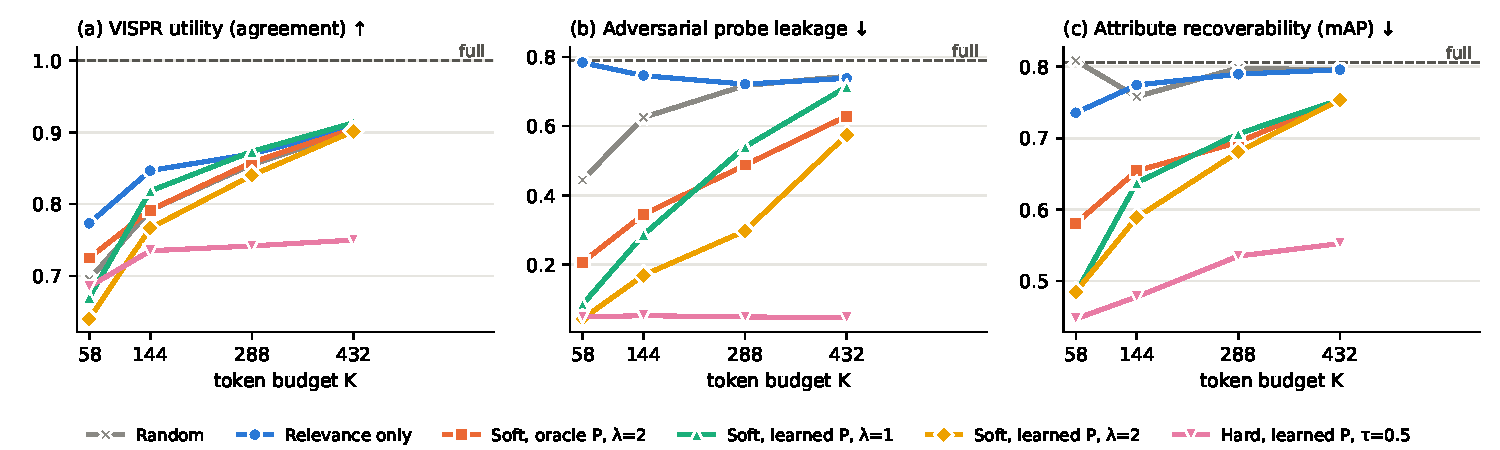
\includegraphics[width=\linewidth]{figs/budget_curves.pdf}
\caption{Utility, adversarial leakage, and recoverability across token budgets (attention relevance). Privacy-aware selection lowers leakage far below
relevance-only pruning at every budget, while recoverability falls much less. The hard gate keeps fewer than $K$ tokens.}
\label{fig:budget}
\end{figure}

\begin{table}[h]
\centering\small
\caption{Paired bootstrap 95\% confidence intervals at $K=288$.}
\label{tab:ci}
\begin{tabular}{@{}llcc@{}}
\toprule
Comparison & Metric & Difference & 95\% CI \\
\midrule
learned $\lambda=1$ vs.\ relevance only & GQA accuracy & $+0.000$ & $[-0.030, +0.030]$ \\
learned $\lambda=1$ vs.\ relevance only & adversarial leakage & $-0.181$ & $[-0.217, -0.143]$ \\
learned $\lambda=2$ vs.\ relevance only & adversarial leakage & $-0.424$ & $[-0.467, -0.382]$ \\
learned $\lambda=2$ vs.\ relevance only & GQA accuracy & $-0.043$ & $[-0.080, -0.007]$ \\
learned $\lambda=2$ vs.\ oracle $\lambda=2$ & adversarial leakage & $-0.190$ & $[-0.230, -0.153]$ \\
\bottomrule
\end{tabular}
\end{table}

\textbf{Relevance-based pruning prefers private content.} Relevance-only pruning keeps \emph{more} private tokens than random pruning
(PTR 0.66 vs.\ 0.49 at $K=288$). At $K=58$ its adversarial leakage (0.78) is nearly that of the full model, while random pruning's is 0.44.
LLaVA's attention concentrates on people and text, which is where VISPR's private attributes are. Attention-based efficiency pruners therefore
act as privacy-\emph{amplifying} filters.

\textbf{Privacy can be bought cheaply at moderate budgets.} With the learned predictor and $\lambda=1$ at $K=288$, GQA accuracy is unchanged
(the confidence interval includes zero), private-token retention falls from 0.66 to 0.20, and adversarial leakage falls by 0.18. With $\lambda=2$,
leakage falls by 0.42 for a small but significant 4-point GQA cost. At $K=144$ the leakage reduction is larger still (0.75 to 0.17), at a 2--4 point GQA cost.
The hard gate reduces leakage to 0.05 at every budget, at a larger utility cost (13 points of VISPR agreement at $K=288$), because it removes every
high-risk token regardless of the question.

\textbf{Removing tokens does not remove information.} With the oracle at $\lambda=2$ and $K=288$, only 7\% of private tokens survive, yet the model
still confirms 49\% of present attributes, and a linear probe recovers attributes with mAP 0.69 (full model 0.81, chance 0.09). Even the hard gate leaves
recoverability at 0.54, six times chance. CLIP's self-attention has already spread information about private regions into other tokens before any pruning happens.

Figure~\ref{fig:qual} shows examples. Relevance-only pruning keeps most of the face, plate, or document tokens when asked about them; privacy-aware
selection removes them, the model can no longer confirm the attribute, and the answer to a neutral question is unchanged.

\begin{figure}[t]
\centering
\includegraphics[width=0.92\linewidth]{figs/qualitative.pdf}
\caption{Tokens kept at $K=288$ for an adversarial probe (``Is someone's face / a person's name / a ticket visible?''); dark regions are dropped.
Titles give the model's answer to the probe and to a neutral question asked separately. Annotated private regions are pixelated for display only;
the model saw the original images.}
\label{fig:qual}
\end{figure}

\subsection{Why the learned predictor beats the ground truth: context tokens}
The learned predictor flags more tokens than the masks (239 vs.\ 166 per image at threshold 0.5), and 36\% of its high-risk tokens lie \emph{outside}
the annotated regions. These are concentrated next to the masks: the share of tokens flagged is 0.93 inside a mask, 0.43 one token away, 0.27 two tokens away,
and 0.15 further away. Working on contextual CLIP features, the predictor has learned that the neighbours of a face also carry the face.

To test this explanation, we dilate the ground-truth masks on the token grid by one or two tokens and repeat the selection (Table~\ref{tab:dil}).
Dilating by one token closes most of the gap: at $K=144$, its adversarial leakage (0.14) is statistically indistinguishable from the learned predictor's
(difference $-0.03$, 95\% CI $[-0.06, +0.01]$), and at $K=288$ it falls from 0.49 to 0.38, though it remains above the learned predictor
(difference $+0.08$, CI $[+0.05, +0.12]$). A substantial part of the leakage therefore sits in tokens adjacent to the annotated regions.

Dilating by two tokens is \emph{worse} than by one. Two-token dilation flags 300 of 576 tokens per image, more than $K=288$ in 56\% of images, so selection must
keep some flagged tokens, and dilation gives the ring the same score as the core, so it cannot prefer ring tokens over core tokens. The learned score is \emph{graded}
(mean 0.89 inside a mask, 0.47 one token away, 0.34 two away), so under a tight budget it gives up the least risky tokens first.
Privacy risk is best modelled as a graded, context-aware score rather than a binary region.

\begin{table}[h]
\centering\small
\caption{Dilating the ground-truth masks ($\lambda=2$, attention relevance). PTR is measured against the undilated masks.}
\label{tab:dil}
\begin{tabular}{@{}clcccc@{}}
\toprule
$K$ & Privacy score & VISPR util.\,$\uparrow$ & PTR\,$\downarrow$ & Adv.\ leak\,$\downarrow$ & Benign leak\,$\downarrow$ \\
\midrule
\multirow{4}{*}{288} & Oracle $P^{GT}$ & 0.86 & 0.07 & 0.49 & 0.44 \\
 & Oracle dilated by 1 token & 0.83 & 0.07 & 0.38 & 0.33 \\
 & Oracle dilated by 2 tokens & 0.85 & 0.12 & 0.48 & 0.44 \\
 & Learned $P$ & 0.84 & 0.13 & 0.30 & 0.27 \\
\midrule
\multirow{4}{*}{144} & Oracle $P^{GT}$ & 0.79 & 0.01 & 0.35 & 0.28 \\
 & Oracle dilated by 1 token & 0.74 & 0.01 & 0.14 & 0.11 \\
 & Oracle dilated by 2 tokens & 0.75 & 0.02 & 0.21 & 0.15 \\
 & Learned $P$ & 0.77 & 0.04 & 0.17 & 0.10 \\
\bottomrule
\end{tabular}
\end{table}

\subsection{Which attributes leak}
Adversarial leakage per attribute at $K=288$, from the full model to the learned predictor with $\lambda=2$: face 0.84 $\to$ 0.10, person 0.96 $\to$ 0.27,
nudity 0.48 $\to$ 0.09, name 0.76 $\to$ 0.35, date/time 0.86 $\to$ 0.53, handwriting 1.00 $\to$ 0.71. Visual attributes are suppressed; text attributes persist,
matching the predictor's weak AP on text (Table~\ref{tab:head}). The ground-truth masks do much worse than the learned predictor on \emph{person}
(0.69 vs.\ 0.27): a person can be recognised from context such as clothing, shadow, and posture, which lies outside a tight polygon.

\subsection{Relevance computed on the device}
With CLIP relevance, which needs no language-model pass, GQA accuracy is unchanged by pruning (0.600 for relevance only at $K=288$; 0.563 with the learned predictor
and $\lambda=1$), but VISPR agreement is 7 points lower than with attention relevance (0.80 vs.\ 0.87), because CLIP similarity localises generic questions such as
``What kind of place is this?'' poorly. Its benign leakage is lower (0.16 vs.\ 0.47 at $\lambda=1$), because CLIP relevance does not concentrate on people the way
the language model's attention does. This is the variant to use when the language model is untrusted.

\subsection{Efficiency}
Privacy is obtained through token removal, so the language model processes $K$ instead of 576 visual tokens; at $K=288$ the input sequence is roughly halved,
and at $K=144$ it shrinks to about a third, with corresponding savings in prefill compute and KV-cache memory. The added cost is small: the privacy predictor is a
0.27M-parameter MLP, attention relevance requires a partial pass through the first 16 of the 32 language-model layers, and CLIP relevance
requires only CLIP's text encoder.
% TODO: add measured prefill / end-to-end latency (scripts/08_latency.py) once the GPU is free.

% =========================================================
\section{Discussion and limitations}
Privacy-aware selection is an effective and essentially free first line of defence: at moderate budgets it removes most private tokens and roughly halves
attribute leakage without hurting standard VQA accuracy. It is not a privacy guarantee. Private information spreads across tokens inside the vision encoder,
so attributes remain recoverable from the kept tokens, and text-based attributes are poorly detected at the token level.

Our evaluation has limitations. (i) The probes test whether the model can \emph{confirm} an attribute; extracting it (e.g.\ reading a name or plate) is a stronger
threat that we have not yet measured. (ii) We evaluate 200 VISPR images, 300 GQA questions, and one VLM; the key differences are statistically significant at this
size, but generality to other models is untested. (iii) The hard gate keeps fewer than $K$ tokens, so it is compared at a slightly lower budget.
(iv) VISPR utility questions are generated from templates; GQA is the more reliable utility measure.

\section{Conclusion and future work}
We showed that visual-token pruning, usually studied for efficiency, can be made privacy-aware with a tiny predictor on frozen features, and that doing so
matters: relevance-based pruning otherwise keeps private content preferentially. We also found that the leakage is partly located around, not only inside,
the private regions, and that removing tokens after the vision encoder leaves private attributes recoverable. Next steps follow directly:
(1) redaction \emph{inside} the vision encoder, blocking attention to high-risk tokens from an intermediate layer so that private content cannot spread;
(2) a text-aware predictor that adds text-detector features for names, addresses, and dates; (3) extraction probes scored against ground-truth text;
(4) comparison with existing pruners (FastV, VisPruner, DivPrune) as relevance estimators; and (5) evaluation on all 2,989 test images, a second VLM,
and a second privacy dataset such as HR-VISPR to test whether the predictor generalises.

\bibliographystyle{plainnat}
\bibliography{refs}

\end{document}
